\newpage


\section{The Muffin vs Chihuahua dataset}\label{sec:the-muffin-vs-chihuahua-dataset}

The Muffin vs Chihuahua set used for the project was published on Kaggle\cite{datasetCite}.
It is made out around six thousand classified images of Muffins and Chihuahuas scraped from google search.
As the data is labeled we can make use of the \textbf{supervised learning} paradigm.

The images in the dataset are of various sizes but all in .jpg format.

\subsection{Data distribution and normalization}
The dataset, by default, is already partitioned in order to have a predetermined test set that is around 20\% of the total data.
Both in training and test sets around 45\% of the images are muffins.
This meas that we have a very small imbalance on the dataset which, by Google's\cite{googleBalance} guidelines, is not concerning.

For the project it was decided to partition the data into:
\begin{itemize}
    \item \textbf{Training set} (70\%): Samples used to train the Neural Network
    \item \textbf{Validation set} (10\%): A split used for two main reasons:
    \begin{itemize}
        \item To measure learning without compromising the test set.\\
        We should not draw conclusions on the learning process on the test set as it is reserved for the final model evaluation.
        \item To apply \textbf{Early Stopping}(\ref{subsec:epochs}) as a regularization technique.

    \end{itemize}
    \item \textbf{Test set} (20\%): Used to evaluate the final obtained model.
\end{itemize}

The reason we use split the dataset into [70,10,20] parts is that it allows to not waste too much data on the validation set while still
keeping the 5-fold CV partitioning as intended for the test split, covering the full dataset.
% todo ref k-foldcv

% todo finisci qui meglio questo

\paragraph{}
An important step when working with data, in order to make the learning process faster and more effective, is preprocessing.
For the project images have been standardized $(\mu=0, \sigma=1)$ as it improves the calculations of the gradients and grants a faster convergence.
%    Uniform Feature Scaling: Normalizing ensures that all features (pixel values) contribute equally to the distance calculations, preventing any single feature from disproportionately influencing the learning process.
%    Improved Gradient Behavior: Normalized data helps maintain a consistent scale of input values, leading to more stable and effective gradient updates during backpropagation. This reduces the risk of issues such as exploding or vanishing gradients.
%    Faster Convergence: When data is normalized, the optimization algorithms (like gradient descent) converge more quickly because the parameters can be adjusted in a more balanced and consistent manner.
%    Reduced Bias in Parameter Initialization: With normalized data, weight initialization schemes can be more effectively applied, which helps in achieving unbiased and efficient learning.
%    Enhanced Data Distribution: Normalization often transforms the data distribution to a standard range (e.g., zero mean and unit variance), which is ideal for many machine learning algorithms, leading to better model performance.

While all images are going to be standardized, to avoid a common pitfall, it is important to calculate the mean($\mu$) and the standard deviation($\sigma$) on the training set alone.
If not done like this we would be having \textit{data leakage} which might lead to overfitting as we also learn from the features of unseen data.

\subsection{Data Augmentation}\label{subsec:data-augmentation}
% todo vedi se la fa ok
Regularization is any modification we make to a learning algorithm that is intended to reduce its generalization error but not its training error.
Data augmentation is a process that falls under these techniques.\cite[Section 5.2.2]{Goodfellow-et-al-2016}

The idea to create more samples with small variations to extend the training set whilst making them valid
is a common practice in computer vision tasks.

% Todo: Faccio vedere il mio modello di augmentaiton
% todo : show images augmented

During the development of the project only the first few models were defined without the use of data augmentation.
They were later enriched with this functionality as it provided a general increase in performance.

The augmentation in \textit{Keras} can be defined as part of the model. The used procedure is the one shown in the graph of the image \ref{fig:custom_aug_proc}.

\begin{figure}[h]
    \centering
    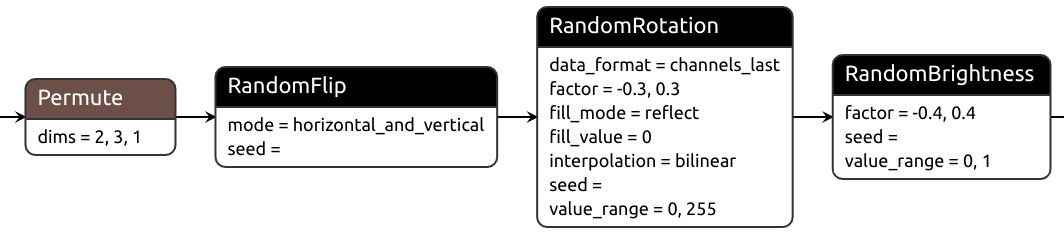
\includegraphics[scale=0.3]{imgs/augmentation_only_model_structure}\\
    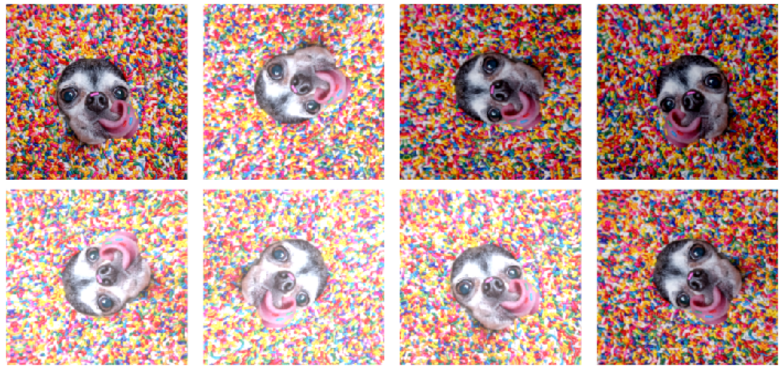
\includegraphics[scale=0.4]{imgs/aug_example_rew}
    \caption{
        The first image shows the augmentation structure used in the project.\\
        Below are shown various transformations done on the same (first of grid) image.
    }\label{fig:custom_aug_proc}
\end{figure}


